\chapter{癌症生物学}\label{ch:b3:cancer-biology}

一个大到能摸到、直径一厘米的\omterm{def:b3:cancer-biology:hallmarks}{肿瘤}，含约十亿个细胞，
是由一个出错的细胞经约三十次倍增而来的，
通常要经过十年左右的生长，人们才会察觉。在这个细胞背后，
有好几次突变，每一次都必须发生在同一谱系之中，
且每一次都摧毁了前两章所讲的一种调控：
分裂的刹车、死亡的触发器、分裂次数的限制，
以及停留原地的要求。\omterm{def:b3:cancer-biology:hallmarks}{癌症}是
细胞群体在体内通过突变和选择而发生的演化，
其结果是一种有利于细胞、却导致生物体死亡的状态。本
章讨论被打击的基因及其正常功能，
讨论揭示需要多少次打击的统计规律，
讨论\omterm{def:b3:cancer-biology:hallmarks}{肿瘤}在超过一毫米并发生扩散时必须获得的生理特征，
讨论可以避免的致病因素，以及生物学已使其成为可能的疗法——从杀伤分裂细胞的毒物，
到释放免疫系统的抗体——
并讨论这些疗法常常失败的
演化原因。

\section{什么是癌症}

\begin{definition}[肿瘤、癌症、癌症的特征]\label{def:b3:cancer-biology:hallmarks}
\index{癌症}\index{肿瘤}\index{恶性}\index{转移}\index{癌症的特征}
\emph{肿瘤}（赘生物）是一群摆脱了生长调控、
并在组织中不断积累的克隆细胞。若其局限于包膜之内，则为\emph{良性}的；
若其细胞侵入邻近组织，并在别处形成继发肿瘤，则为\emph{恶性}的——
即\emph{癌症}。这种继发肿瘤的形成过程称为
\emph{转移}，正是它致人死亡。
癌症以其起源细胞命名：源自上皮的癌
（占人类癌症的 \qty{85}{\%}），源自结缔组织的肉瘤，
源自造血细胞的白血病和淋巴瘤，源自神经胶质的胶质瘤。
无论发生在哪种组织，恶性克隆都获得了同一组能力，
即\emph{癌症的特征}：它在没有外部生长信号的情况下增殖，并无视本应使其停止的信号；
它抵抗\omterm{def:b3:cell-cycle-apoptosis:apoptosis}{细胞凋亡}；
它在\omterm{def:b3:cancer-biology:telomerase}{端粒酶}被重新激活后无限分裂；
它诱导\omterm{prop:b3:cancer-biology:oxygen}{血管生成}；它\omterm{def:b3:cancer-biology:metastasis}{侵袭}并发生转移；
在这些能力之下，其基因组不稳定，
代谢\omterm{def:b3:chromatin-epigenetics:epigenetics}{重编程}为糖酵解，即使在有氧条件下也如此（瓦伯格效应）；
它还招募有助于自身的炎症细胞，并逃避免疫系统的攻击。
每一项特征都意味着正常组织的某种调控被攻破，
并可对应到某个基因上。
\end{definition}

\begin{omfigure}
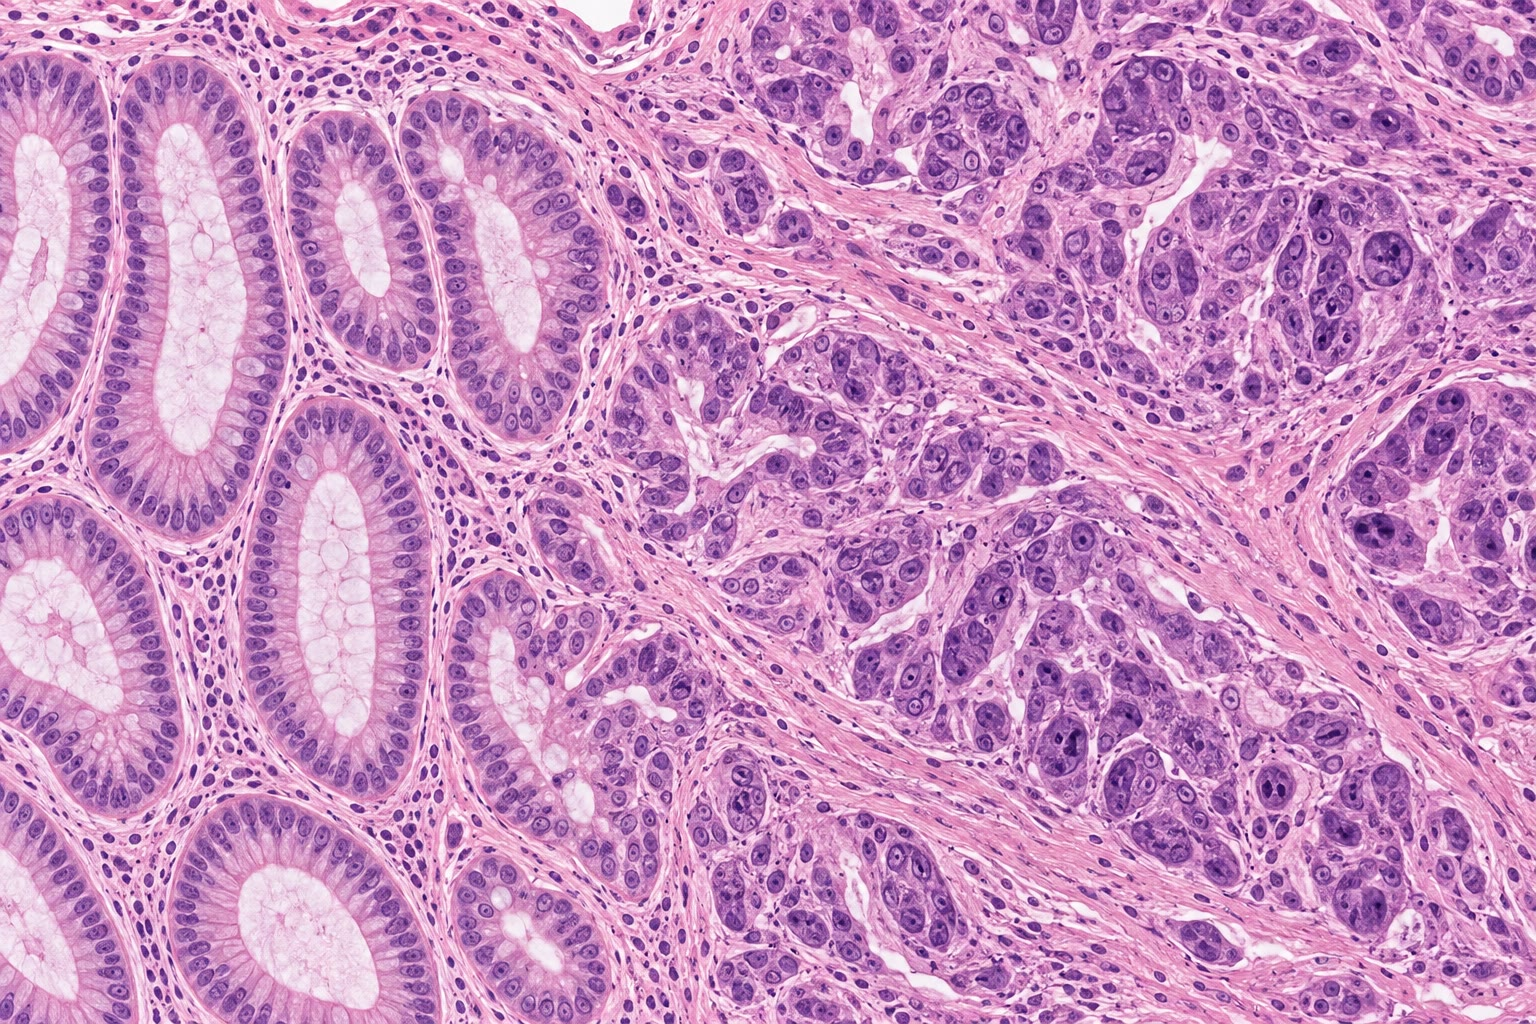
\includegraphics[width=0.56\linewidth]{images/book5/ai/b5-11-tumour-histology.jpg}

{\small 癌的边缘：左侧为排列有序的腺上皮，细胞核形态规则；
右侧为拥挤的细胞，细胞核大而形态不规则，
正侵入下方的基质——
病理学家据此判断\omterm{def:b3:cancer-biology:hallmarks}{肿瘤}为\omterm{def:b3:cancer-biology:hallmarks}{恶性}。}
\end{omfigure}

\section{被打击的基因}

\begin{definition}[癌基因与肿瘤抑制基因]\label{def:b3:cancer-biology:genes}
\index{癌基因}\index{原癌基因}\index{肿瘤抑制基因}\index{Ras}\index{p53}\index{二次打击假说}
\emph{原癌基因}是促进增殖或存活的正常基因，
如生长因子、其受体、信号蛋白、转录因子、周期蛋白；
\emph{癌基因}则是在没有正常信号时仍保持活性的突变形式：
例如点突变使小 GTP 酶\emph{Ras}锁定在 GTP 状态（
第 12 位甘氨酸，占全部\omterm{def:b3:cancer-biology:hallmarks}{癌症}的四分之一），
受体基因 HER2 或转录因子基因 Myc 的扩增，
以及在慢性粒细胞白血病中使\emph{BCR}与激酶\emph{ABL}融合的易位，
或是在伯基特淋巴瘤中使\emph{MYC}紧邻抗体增强子的易位。
一个突变等位基因即已足够：癌基因以显性方式起作用。
\emph{\omterm{def:b3:cancer-biology:hallmarks}{肿瘤}抑制基因}抑制增殖、促进死亡或修复，
例如\omterm{def:b3:cell-cycle-apoptosis:checkpoints}{限制点}处的 Rb 和 p16、守护基因\emph{p53}
（它使受损细胞停滞或将其杀死）、结肠 Wnt 通路中的 APC、
PTEN、BRCA1 和 BRCA2，以及\omterm{prop:b3:dna-repair:fidelity}{错配修复}基因。
它必须两个等位基因都丢失才会起作用：即\emph{二次打击}，
其中第一次常在家族性\omterm{def:b3:cancer-biology:hallmarks}{癌症}综合征中遗传，
第二次则为体细胞突变。\emph{p53}在半数人类\omterm{def:b3:cancer-biology:hallmarks}{癌症}中发生突变，
其通路在其余大多数\omterm{def:b3:cancer-biology:hallmarks}{癌症}中
失效。
\end{definition}

\begin{proof}[证据]
劳斯（1911）用无细胞滤液传播了一种鸡肉瘤，
滤液中含一种病毒，其唯一的转化基因\emph{src}经
瓦慕斯和毕晓普（1976）证明，是正常鸡基因的一个被捕获的拷贝
——\omterm{def:b3:cancer-biology:genes}{癌基因}是被改变了的细胞基因。温伯格（1982）将人膀胱癌的
DNA 转入培养的小鼠细胞，使其发生转化；
起作用的片段为\emph{RAS}，其中有一个碱基改变，
且该改变在患者的正常组织中不存在。
克努森（1971）比较了患视网膜母细胞瘤（一种眼部\omterm{def:b3:cancer-biology:hallmarks}{肿瘤}）的儿童：
有家族病史者双眼多发\omterm{def:b3:cancer-biology:hallmarks}{肿瘤}，且发病早；
无家族病史者仅发生一个\omterm{def:b3:cancer-biology:hallmarks}{肿瘤}，且发病较晚。
这与家族性病例只需一次体细胞事件、散发性病例需两次相符，
也与一个必须两个拷贝都丢失的基因相符。\emph{RB}于
1986 年被克隆，并在每一个\omterm{def:b3:cancer-biology:hallmarks}{肿瘤}中证实
两个等位基因确实都已失活。
\end{proof}

\begin{theorem}[打击次数与年龄曲线]\label{thm:b3:cancer-biology:armitage-doll}
\index{阿米蒂奇–多尔模型}\index{多阶段致癌}
设某种\omterm{def:b3:cancer-biology:hallmarks}{癌症}需要在同一细胞谱系中发生 $k$ 个独立的限速事件，
每个事件以每个细胞每年 $u$ 的恒定速率发生，
细胞群体含 $N$ 个易感细胞，且 $ut \ll 1$。则
某一细胞已经历全部 $k$ 个事件（至年龄 $t$）的概率
约为 $(ut)^{k}$，组织中的累积风险约为 $N(ut)^{k}$，
而发病率——即年龄 $t$ 时每年的新病例数——为
\[
I(t) \approx N\,k\,u^{k}\,t^{\,k-1},
\]
是年龄的幂函数，指数为 $k - 1$，在双对数图上为斜率为 $k - 1$ 的直线。
对于遗传了其中一个事件的个体，
同一\omterm{def:b3:cancer-biology:hallmarks}{癌症}的发病率 $\propto t^{\,k-2}$，幂次降低一次。
\end{theorem}
\begin{proof}
每个事件以速率 $u$ 发生，到时刻 $t$ 已发生的概率为
$1 - e^{-ut} \approx ut$；各事件相互独立，因此全部 $k$ 个事件都已发生的概率为
$(ut)^{k}$，而事件发生的先后次序在此无关紧要。
细胞数为 $N$，事件罕见，
故完成整个序列的细胞期望数
为 $N(ut)^{k}$，发病率即其时间导数 $Nku^{k}t^{k-1}$。
若已遗传一个事件，则还需发生 $k - 1$ 个：
$(ut)^{k-1}$，发病率 $\propto t^{k-2}$。若事件的先后顺序有影响（仅 $1$ 种
顺序导致\omterm{def:b3:cancer-biology:hallmarks}{癌症}，共 $k!$ 种），则前置因子会改变，而指数不变。
\end{proof}

\begin{example}[读懂指数]\label{ex:b3:cancer-biology:exponent}
大多数成人癌的发病率大致随年龄的五到
六次方增长——从三十岁时每年约 $1$ 例 / \num{100000} 人，
到八十岁时约 $1$ 例 / $300$ 人，发病率增加 $300$ 倍，年龄则增加 $2.7$ 倍，
$2.7^{5.7} \approx 300$——这提示需要六到七
个限速事件。这一估计比较粗略：克隆在每次打击之后的扩增
会增加下一次打击的风险细胞数，因此克隆生长穿插其间时，
较少的事件也能给出相同的斜率，而在测序的\omterm{def:b3:cancer-biology:hallmarks}{肿瘤}中发现的
\emph{驱动}突变数目为两到
八个。克努森的视网膜母细胞瘤恰好符合定理的第二个陈述：
散发型疾病需要两次打击，其发病率
随年龄上升（在视网膜母细胞存在的数年内）；遗传型疾病
只需一次打击，自出生起即以近乎恒定的速率出现，
且发病早、反复发生。
\end{example}

\begin{omfigure}
\begin{tikzpicture}
\begin{axis}[
  width=0.68\linewidth, height=6cm,
  xmode=log, ymode=log,
  xmin=20, xmax=100, ymin=1e-6, ymax=1e-1,
  xlabel={年龄（岁）}, ylabel={每人每年发病率},
  xlabel style={font=\small, at={(axis description cs:0.5,-0.12)}, anchor=north},
  ylabel style={font=\small},
  tick label style={font=\small}, xtick={20,30,50,80}, xticklabels={20,30,50,80},
  clip=false,
]
\addplot[very thick, omThm, domain=20:100, samples=2] {1e-5*(x/30)^5.7};
\addplot[very thick, omDef, domain=20:100, samples=2] {3e-4*(x/30)^1};
\addplot[very thick, omMeth!70!black, domain=20:100, samples=2] {2e-3};
\node[font=\scriptsize, omThm, anchor=south west] at (axis cs:38,2.5e-6) {癌：斜率 $5$--$6$，六到七次事件};
\node[font=\scriptsize, omDef, anchor=south west] at (axis cs:22,6e-4) {两次打击：斜率 1};
\node[font=\scriptsize, omMeth!70!black, anchor=south west] at (axis cs:22,2.3e-3) {遗传一次打击：斜率 0};
\end{axis}
\end{tikzpicture}

{\small 发病率随年龄变化的对数坐标图。需要 $k$
个限速事件的\omterm{def:b3:cancer-biology:hallmarks}{癌症}，其发病率按 $t^{k-1}$ 增长：成人癌的陡峭直线，
以及克努森的两种情形——两次打击的\omterm{def:b3:cancer-biology:hallmarks}{肿瘤}呈线性增长，
而携带一次遗传打击者的同一\omterm{def:b3:cancer-biology:hallmarks}{肿瘤}则
自出生起以恒定速率发生。}
\end{omfigure}

\begin{proposition}[被打击的通路]\label{prop:b3:cancer-biology:pathways}
\index{Ras--MAPK 通路}\index{PI3K 通路}\index{Wnt 通路}
数百个\omterm{def:b3:cancer-biology:genes}{癌基因}归入十余条通路，每条通路
都会在某一环节被\omterm{def:b3:cancer-biology:hallmarks}{肿瘤}破坏。生长因子通路：受体
酪氨酸激酶（EGFR、HER2）、\omterm{def:b3:cancer-biology:genes}{Ras}，激酶级联 Raf--MEK--ERK 通向
细胞核，与之并联的 PI3K--Akt--mTOR 通向存活与生长，
受 PTEN 抑制；\omterm{def:b3:cancer-biology:hallmarks}{肿瘤}只需激活其中之一，无论是哪个基因。
\omterm{def:b3:cell-cycle-apoptosis:cdk}{细胞周期}的刹车：周期蛋白 D、Cdk4、p16、Rb（见\cref{ch:b3:cell-cycle-apoptosis}）。
守护者：\omterm{def:b3:cancer-biology:genes}{p53} 及其调节因子。死亡：Bcl-2。发育信号：
结肠中的 Wnt（APC、$\beta$-连环蛋白），皮肤
和脑中的 Hedgehog，T~细胞中的 Notch。基因组维持：\omterm{prop:b3:dna-repair:fidelity}{错配修复}、
\omterm{def:b3:dna-repair:dsb}{BRCA}、\omterm{def:b3:dna-repair:ddr}{ATM}。\omterm{def:b3:chromatin-epigenetics:nucleosome}{染色质}：
在\cref{ch:b3:chromatin-epigenetics}中的\omterm{def:b3:chromatin-epigenetics:histone-code}{书写器}与重塑因子，约三分之一的\omterm{def:b3:cancer-biology:hallmarks}{肿瘤}发生突变。
永生化：\omterm{def:b3:cancer-biology:telomerase}{端粒酶}启动子。由于通路是一系列
步骤，不同基因的突变互为替代——携带突变型 \omterm{def:b3:cancer-biology:genes}{Ras} 的\omterm{def:b3:cancer-biology:hallmarks}{肿瘤}
很少同时携带突变型 EGFR——针对某一步骤的药物，
可能被其下游的突变所击败。
\end{proposition}

\begin{omfigure}
\begin{tikzpicture}[every node/.style={font=\scriptsize}, >=stealth]
  % membrane
  \draw[very thick, omDef] (0,3.6) -- (12,3.6); \draw[very thick, omDef] (0,3.3) -- (12,3.3);
  \node[above] at (1.0,3.65) {细胞外}; \node[below] at (1.0,3.25) {细胞质};
  % receptor
  \draw[thick, fill=omProp!35] (3.7,3.0) rectangle (4.1,4.1); \draw[thick, fill=omProp!35] (4.3,3.0) rectangle (4.7,4.1);
  \node[above, align=center] at (4.2,4.15) {生长因子 $\to$ 受体激酶 \\(EGFR, HER2)}; \node[right, omThm, font=\tiny] at (4.75,4.0) {扩增};
  % Ras
  \node[draw, thick, rounded corners, fill=omDef!20] (ras) at (4.2,2.3) {活化的 Ras--GTP};
  \node[right, omThm, font=\tiny] at (5.5,2.3) {G12：持续激活};
  \node[draw, thick, rounded corners, fill=omDef!20] (raf) at (4.2,1.4) {Raf $\to$ MEK $\to$ ERK 级联};
  \node[right, omThm, font=\tiny] at (5.8,1.4) {BRAF V600E 突变};
  \node[draw, thick, rounded corners, fill=omMeth!25] (myc) at (4.2,0.4) {Myc、周期蛋白 D：增殖};
  \node[right, omThm, font=\tiny] at (6.4,0.4) {Myc 扩增};
  \draw[->, thick] (4.2,3.0) -- (ras); \draw[->, thick] (ras) -- (raf); \draw[->, thick] (raf) -- (myc);
  % PI3K branch
  \node[draw, thick, rounded corners, fill=omDef!20] (pi3k) at (9.6,2.3) {PI3K $\to$ Akt $\to$ mTOR 通路};
  \node[draw, thick, rounded corners, fill=omMeth!25] (surv) at (9.6,0.4) {存活、生长};
  \draw[->, thick] (4.7,3.0) .. controls (6.5,2.8) .. (pi3k.north west); \draw[->, thick] (pi3k) -- (surv);
  \node[draw, thick, rounded corners, fill=omThm!15] (pten) at (12.2,1.4) {PTEN 基因}; \draw[-|, thick, omThm] (pten) -- (9.6,1.4);
  \node[below, omThm, font=\tiny] at (12.2,1.15) {缺失};
  % p53 and Rb on the side
  \node[draw, thick, rounded corners, fill=omThm!15] (rb) at (1.2,0.4) {Rb、p16 基因}; \draw[-|, thick, omThm] (rb) -- (myc);
  \node[below, omThm, font=\tiny, align=center] at (1.2,0.15) {两个等位基因均丢失};
  \node[draw, thick, rounded corners, fill=omThm!15] (p53) at (1.2,1.6) {p53}; \node[below, omThm, font=\tiny, align=center] at (1.2,1.35) {约一半 \\癌症中发生突变};
  \draw[-|, thick, omThm] (p53) -- (1.2,0.65);
\end{tikzpicture}

{\small 生长因子通路及\omterm{def:b3:cancer-biology:hallmarks}{癌症}打击的位置。绿色
方框为输出，蓝色为致癌突变锁定的信号步骤，
红色为\omterm{def:b3:cancer-biology:hallmarks}{肿瘤}丢失的抑制因子（竖线表示
抑制）。该图中，一个\omterm{def:b3:cancer-biology:hallmarks}{肿瘤}通常携带一个激活性\omterm{def:b3:dna-repair:lesions}{损伤}和一到两个
失活性\omterm{def:b3:dna-repair:lesions}{损伤}。}
\end{omfigure}

\section{肿瘤的演化}

\begin{proposition}[多步致癌作用]\label{prop:b3:cancer-biology:multistep}
\index{驱动突变}\index{乘客突变}\index{克隆演化}\index{突变特征}
\omterm{def:b3:cancer-biology:hallmarks}{肿瘤}是体细胞演化的产物：突变产生变异，
组织内的选择有利于分裂更快、
死亡更少或摆脱约束的变异。结直肠序列
由福格尔斯坦阐明，是范例：\emph{APC} 缺失产生
一个小的良性息肉；\emph{KRAS} 突变使其长成
腺瘤；\emph{SMAD4} 或 \emph{TP53} 缺失使其转化为癌；
进一步的变化使其能够\omterm{def:b3:cancer-biology:metastasis}{侵袭}。每一步都是一次克隆扩增，
使下一次打击的风险细胞数倍增。一个测序的\omterm{def:b3:cancer-biology:hallmarks}{肿瘤}携带数以千计的突变，
其中少数——通常为两到八个——
是赋予选择优势的\emph{驱动}突变；其余为
\emph{乘客}突变，随克隆一同携带，其谱型是
记录了致其产生的原因：相邻嘧啶上的 C$\to$T，
黑色素瘤中为紫外线所致，肺癌中 G$\to$T 为烟草烟雾所致，
以及 APOBEC 酶、\omterm{prop:b3:dna-repair:fidelity}{错配修复}缺陷、
黄曲霉毒素留下的印记——即\emph{\omterm{prop:b3:cancer-biology:multistep}{突变特征}}。\omterm{def:b3:cancer-biology:hallmarks}{肿瘤}
是异质性的，呈分支状的亚克隆树，而致死的亚克隆
在诊断时往往只占少数。
\end{proposition}

\begin{omfigure}
\begin{tikzpicture}[every node/.style={font=\scriptsize}, >=stealth]
  \foreach \x/\lab/\gene/\col/\r in {0/正常上皮/{}/omDef!20/0.5, 2.6/小息肉/{APC 丢失（两个等位基因）}/omDef!35/0.7, 5.4/腺瘤/{KRAS 激活}/omProp!40/1.0, 8.4/癌/{SMAD4 或 TP53 丢失}/omThm!35/1.3, 11.6/{浸润、转移}/{更多驱动突变，\\基因组不稳定}/omThm!60/1.5} {
    \draw[thick, fill=\col] (\x,0) circle (\r);
    \node[below, align=center] at (\x,-1.6) {\lab};
    \node[above, align=center, omThm] at (\x,1.6) {\gene};
  }
  \foreach \a/\b in {0.5/1.9, 3.3/4.4, 6.4/7.1, 9.7/10.1} \draw[->, very thick] (\a,0) -- (\b,0);
  \node[below] at (5.8,-2.3) {十到三十年；每一步都是一次克隆扩增，使下一次打击的风险细胞数倍增};
\end{tikzpicture}

{\small 结直肠序列。每一次\omterm{prop:b3:cancer-biology:multistep}{驱动突变}都会扩增一个克隆，
而扩增后的克隆为下一个\omterm{prop:b3:cancer-biology:multistep}{驱动突变}提供了可能发生的细胞，
整个过程历时数十年，因此筛查息肉
可以预防\omterm{def:b3:cancer-biology:hallmarks}{癌症}。}
\end{omfigure}

\begin{method}[Ames 试验]\label{met:b3:cancer-biology:ames}
\index{Ames 试验}\index{诱变剂}
用于检验某化学物质是否具有诱变性，从而推断其是否可能为
\omterm{prop:b3:cancer-biology:causes}{致癌物}：(1) 取一株 \emph{Salmonella} 菌株，
其组氨酸生物合成基因带有点突变，缺少组氨酸便无法生长；
(2) 将待测化学物质与肝脏提取物混合，肝脏中的酶可将许多化合物
转化为具有诱变活性的形式，与机体内的情形一样；(3)
将约 $10^{8}$ 个细菌与该混合物一同涂布于无组氨酸的琼脂平板上；
(4) 计数生长出的菌落——每个菌落都是回复突变体，其中某一新突变恢复了该基因；
(5) 与自发突变率比较。
若回复突变体数随剂量增加而增多，
则表明该化合物会引起点突变。大多数已知\omterm{prop:b3:cancer-biology:causes}{致癌物}的检测结果为阳性；该试验成本低廉，
仅需两天，未通过试验的化合物
在投入生产前还需进一步检验。
\end{method}

\begin{definition}[永生与不稳定性]\label{def:b3:cancer-biology:telomerase}
\index{端粒酶}\index{染色体不稳定性}\index{非整倍性!在癌症中}
正常体细胞不含端粒酶，并以端粒长度计数分裂次数
（见\cref{ch:b3:stem-cells}）：约分裂五十次后细胞\omterm{def:b3:cell-cycle-apoptosis:other}{衰老}；
若细胞因丢失 \omterm{def:b3:cancer-biology:genes}{p53} 和 Rb 而绕过\omterm{def:b3:cell-cycle-apoptosis:other}{衰老}，则会继续分裂，
直至端粒耗尽、染色体融合并断裂——这一危机会杀死大多数克隆。
罕见的存活者重新激活了
\emph{端粒酶}，通常由启动子突变引起，因而获得永生；
\qty{90}{\%} 的\omterm{def:b3:cancer-biology:hallmarks}{癌症}表达该酶。危机会留下痕迹：
染色体融合、断裂，并出现扩增、缺失与易位
——\emph{染色体不稳定性}，伴随纺锤体\omterm{def:b3:cell-cycle-apoptosis:checkpoints}{检查点}的丧失，
以及 \omterm{def:b3:cancer-biology:genes}{p53} 对错误分离应答的丧失，使大多数实体瘤
呈非整倍体，并使其持续产生变异。少数
\omterm{def:b3:cancer-biology:hallmarks}{肿瘤}则因\omterm{prop:b3:dna-repair:fidelity}{错配修复}缺失而具有突变表型，
核型正常，点突变率却高出千倍。
\end{definition}

\section{作为组织的肿瘤}

\begin{proposition}[氧气决定无血管肿瘤的大小]\label{prop:b3:cancer-biology:oxygen}
\index{血管生成}\index{扩散极限}\index{缺氧}
考虑单位体积以恒定速率 $q$ 消耗氧气的组织，
氧气由扩散（扩散系数为 $D$）自血管供给，血管壁处的浓度为
$c_{0}$。在一维稳态下，$D\,
\mathrm{d}^{2}c/\mathrm{d}x^{2} = q$，故 $c(x) = c_{0} - qx^{2}/2D$，氧气在距离
处耗尽，其表达式为
\[
L = \sqrt{\frac{2Dc_{0}}{q}} .
\]
取 $D = \qty{2e-9}{m^2/s}$，$c_{0} = \qty{0.05}{mol/m^3}$ 与 $q =
\qty{0.03}{mol/m^3/s}$（一个进行呼吸的\omterm{def:b3:cancer-biology:hallmarks}{肿瘤}），$L \approx \qty{80}{\micro
m}$：任何细胞距毛细血管都不能超过约一百微米。
因此，一个没有自身血管的克隆在直径达一至两毫米时便停止生长，
其中心\omterm{def:b3:cell-cycle-apoptosis:apoptosis}{坏死}、边缘存活。若要继续生长，它必须诱导\emph{\omterm{prop:b3:cancer-biology:oxygen}{血管生成}}——
即其缺氧细胞使转录因子 HIF 稳定，
HIF 诱导 VEGF 表达，
VEGF 使附近的内皮细胞向其方向出芽。
Judah Folkman 于 1971 年提出，阻断这一步骤即可使\omterm{def:b3:cancer-biology:hallmarks}{肿瘤}“饿死”；
针对 VEGF 的抗体现已成为多种\omterm{def:b3:cancer-biology:hallmarks}{癌症}的标准疗法，
但\omterm{def:b3:cancer-biology:hallmarks}{肿瘤}会产生适应。
\end{proposition}
\begin{proof}
稳态时，扩散通量 $-D\,\mathrm{d}c/\mathrm{d}x$ 必须
随 $x$ 的变化恰好与氧气的消耗速率相同：$\mathrm{d}(-D\,
\mathrm{d}c/\mathrm{d}x)/\mathrm{d}x = -q$，即 $D c'' = q$。
两次积分时，取 $c(0) = c_{0}$ 与 $c'(L) = 0$（在氧气耗尽的深度处，其外不再有通量），
得 $c = c_{0} - qx^{2}/2D$，
再利用 $c(L) = 0$ 确定 $L$。数值由此得出。
\end{proof}

\begin{omfigure}
\begin{tikzpicture}
\begin{axis}[
  width=0.6\linewidth, height=5.4cm,
  axis x line=bottom, axis y line=left,
  xmin=0, xmax=120, ymin=0, ymax=0.06,
  xlabel={距毛细血管的距离 ($\unit{\micro m}$)}, ylabel={氧气 ($\unit{mol/m^3}$)},
  xlabel style={font=\small, at={(axis description cs:0.5,-0.12)}, anchor=north},
  ylabel style={font=\small},
  tick label style={font=\small}, xtick={0,40,80,120}, ytick={0,0.025,0.05},
  clip=false,
]
\addplot[very thick, omDef, domain=0:81.6, samples=40] {0.05 - 0.03*(x*1e-6)^2/(2*2e-9)};
\addplot[very thick, omDef, domain=81.6:120, samples=2] {0};
\fill[omThm!25] (axis cs:81.6,0) rectangle (axis cs:120,0.06);
 \node[font=\scriptsize, omThm!70!black, anchor=south, align=center] at (axis cs:100,0.03) {无氧：\\坏死};
\node[font=\scriptsize, omDef, anchor=south west] at (axis cs:5,0.052) {$c(x) = c_{0} - qx^{2}/2D$};
\draw[dashed, gray] (axis cs:81.6,0) -- (axis cs:81.6,0.06); \node[font=\scriptsize, anchor=south west] at (axis cs:83,0.002) {$L$};
\end{axis}
\end{tikzpicture}

{\small 在进行呼吸的组织中，氧气浓度随距最近毛细血管的距离呈抛物线下降，
并在 $L = \sqrt{2Dc_{0}/q}$ 处耗尽，约为 \qty{80}{\micro m}。
无血管的\omterm{def:b3:cancer-biology:hallmarks}{肿瘤}即是一层厚度为该值的存活细胞，
围绕着死亡的核心。}
\end{omfigure}

\begin{omfigure}
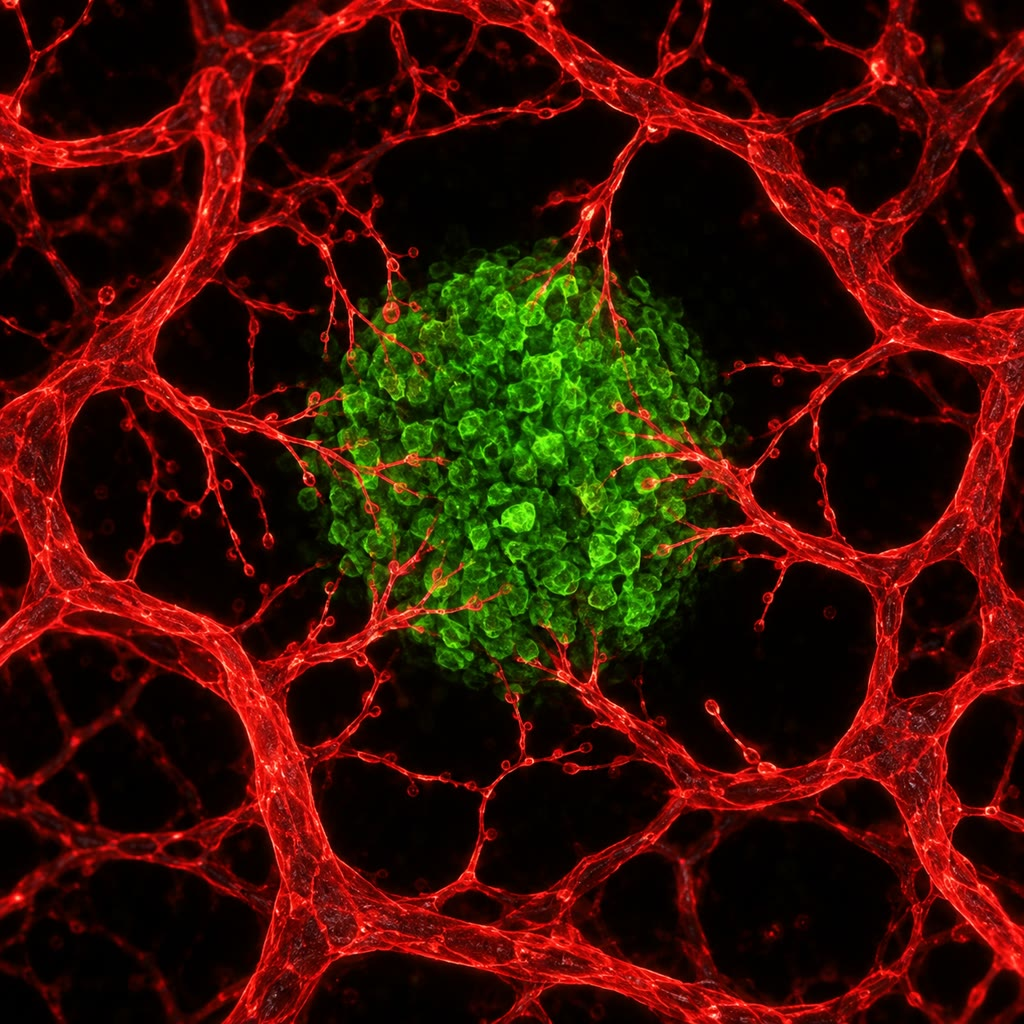
\includegraphics[width=0.36\linewidth]{images/book5/ai/b5-11-angiogenesis.jpg}\hspace{0.04\linewidth}
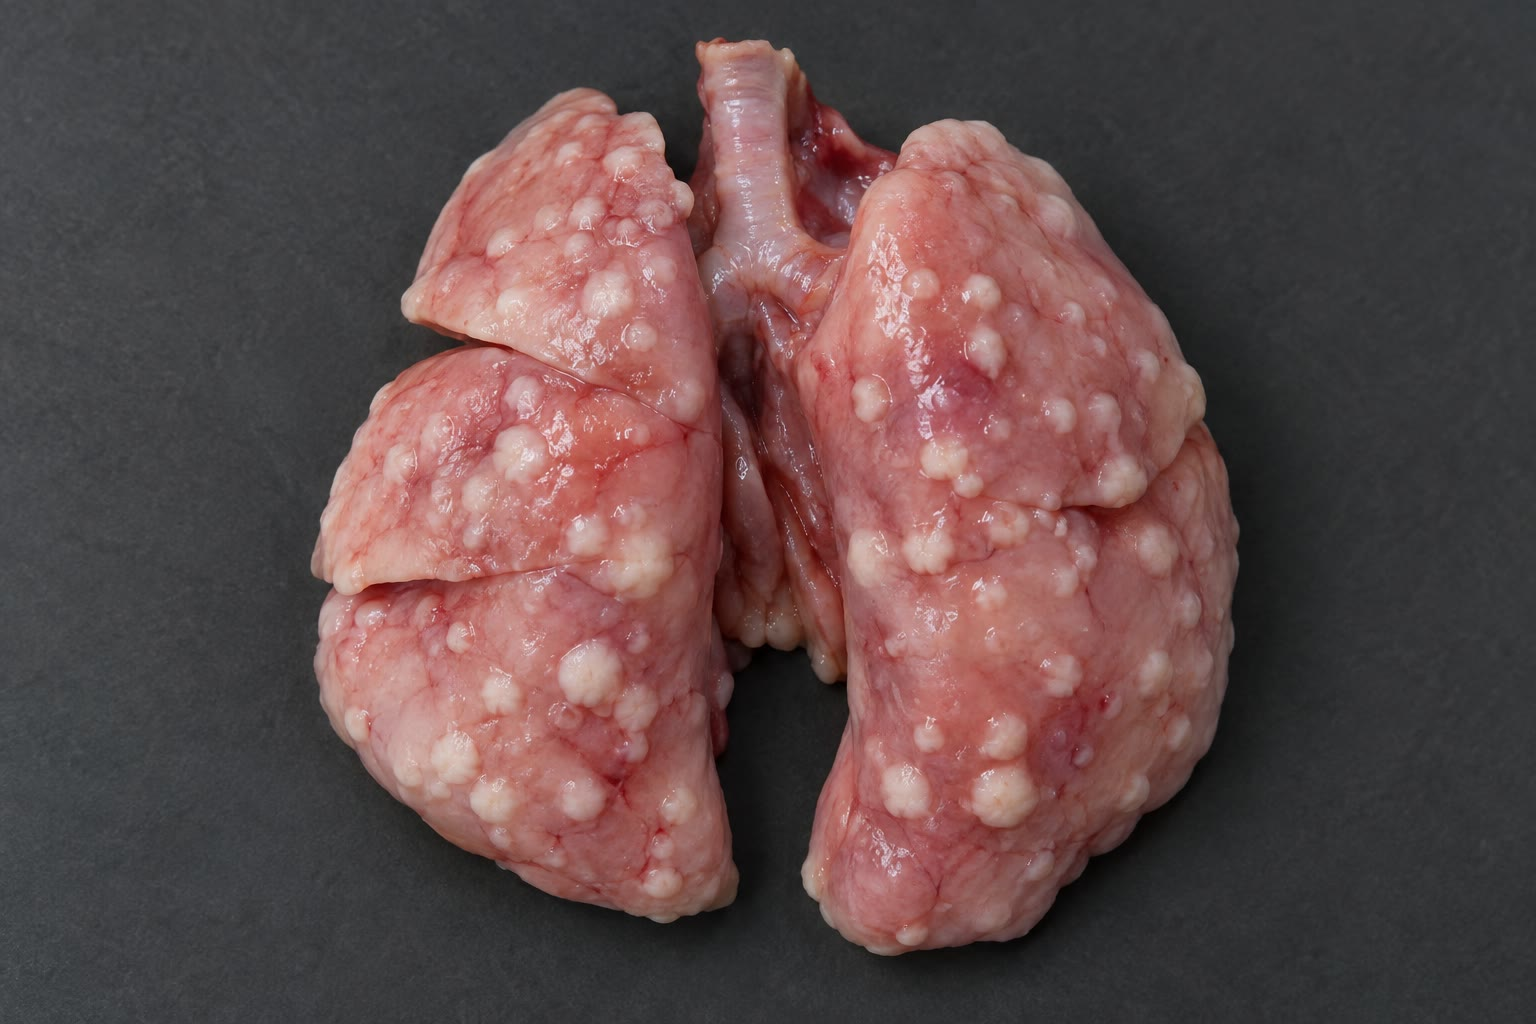
\includegraphics[width=0.54\linewidth]{images/book5/ai/b5-11-metastasis-lung.jpg}

{\small 左图：\omterm{def:b3:cancer-biology:hallmarks}{肿瘤}球体（绿色）从邻近血管网络招募新血管（红色）
——即培养条件下的\omterm{prop:b3:cancer-biology:oxygen}{血管生成}。右图：小鼠肺部布满\omterm{def:b3:cancer-biology:hallmarks}{转移}灶，
每个菌落都由一个
在血液循环中存活下来的细胞建立。}
\end{omfigure}

\begin{definition}[侵袭与转移]\label{def:b3:cancer-biology:metastasis}
\index{侵袭}\index{上皮–间质转化}\index{种子与土壤}
要发生\omterm{def:b3:cancer-biology:hallmarks}{转移}，癌细胞必须离开上皮——
丧失细胞连接和极性，获得运动能力，这一过程即
\emph{上皮–间质转化}，由胚胎发育中通常使用的转录因子驱动——
降解基底膜和基质，
借助分泌的蛋白酶穿过血管或淋巴管壁，
在循环中存活（能够存活的不足万分之一，它们会被剪切力、
缺乏附着以及自然杀伤细胞消灭），
停留在另一器官的毛细血管床中，穿出血管，
并在那里生长。\omterm{def:b3:cancer-biology:hallmarks}{转移}的部位并非随机：乳腺癌\omterm{def:b3:cancer-biology:hallmarks}{转移}至骨、肺、肝和脑，
结肠癌\omterm{def:b3:cancer-biology:hallmarks}{转移}至肝，前列腺癌\omterm{def:b3:cancer-biology:hallmarks}{转移}至骨——
即帕吉特于 1889 年提出的\emph{种子与土壤}学说，该学说
一部分由血流解释，另一部分由细胞与组织信号之间的匹配关系解释。
播散的细胞可能休眠数年后才开始生长，
这也是\omterm{def:b3:cancer-biology:hallmarks}{癌症}在看似治愈十年后复发的原因。
实体瘤导致的死亡中有九成源于\omterm{def:b3:cancer-biology:hallmarks}{转移}，
而\omterm{def:b3:cancer-biology:hallmarks}{转移}也是目前理解最少的环节。
\end{definition}

\begin{proposition}[逃避免疫系统]\label{prop:b3:cancer-biology:immune}
\index{免疫逃逸}\index{检查点抑制剂}\index{新抗原}
\omterm{def:b3:cancer-biology:hallmarks}{肿瘤}的突变会产生\emph{\omterm{prop:b3:cancer-biology:immune}{新抗原}}，即正常细胞不呈递的肽段，
细胞毒性 T~细胞能够识别并杀伤\omterm{def:b3:cancer-biology:hallmarks}{肿瘤}细胞——
这正是免疫抑制患者\omterm{def:b3:cancer-biology:hallmarks}{癌症}更多的原因，
也是突变很多的\omterm{def:b3:cancer-biology:hallmarks}{肿瘤}（黑色素瘤、肺癌、\omterm{prop:b3:dna-repair:fidelity}{错配修复}缺陷的结肠癌）
对免疫疗法应答最好的原因。临床上可见的\omterm{def:b3:cancer-biology:hallmarks}{肿瘤}，都是已逃逸的：
通过丢失呈递肽段的 MHC 分子，
通过分泌抑制性因子，通过招募调节性 T~细胞，
尤其是通过表达 PD-L1——它与 T~细胞上的抑制性受体 PD-1 结合，
使其失效，
这与正常终止免疫应答的刹车机制相同（见\cref{ch:b3:adaptive-immunity}）。
阻断 PD-1 或 PD-L1 的抗体，
或更早发现的刹车分子 CTLA-4 的抗体，可以解除 T~细胞的抑制；在一部分患者中——
依\omterm{def:b3:cancer-biology:hallmarks}{肿瘤}类型不同，占五分之一到一半——
它们能使原本无法治疗的\omterm{def:b3:cancer-biology:hallmarks}{癌症}获得持久缓解，
而其副作用则是自身免疫，即刹车的另一种功能。
\end{proposition}

\section{病因与治疗}

\begin{proposition}[病因]\label{prop:b3:cancer-biology:causes}
\index{致癌物}\index{致癌病毒}
凡是提高定理中所述事件发生速率的
因素，或增加有风险细胞数量的因素，都会导致\omterm{def:b3:cancer-biology:hallmarks}{癌症}。\emph{化学\omterm{prop:b3:cancer-biology:causes}{致癌物}}，
其中多数在肝脏活化后具有诱变性：
烟草烟雾中的七十种\omterm{prop:b3:cancer-biology:causes}{致癌物}导致三分之一的\omterm{def:b3:cancer-biology:hallmarks}{癌症}死亡，
并使肺癌风险升高十五至二十五倍；霉变谷物中的黄曲霉毒素；石棉
虽非\omterm{met:b3:cancer-biology:ames}{诱变剂}，却是一种慢性刺激物。\emph{辐射}：紫外线导致皮肤癌
（\cref{ch:b3:dna-repair}中的二聚体），
电离辐射导致白血病、甲状腺癌和乳腺癌。\emph{感染}，占全球\omterm{def:b3:cancer-biology:hallmarks}{癌症}的六分之一：
乳头瘤病毒，其蛋白 E6 破坏 \omterm{def:b3:cancer-biology:genes}{p53}，E7 使 Rb 失活，
几乎导致所有宫颈癌（现已有疫苗可预防）；
乙型和丙型肝炎病毒导致肝癌；EB 病毒导致淋巴瘤；
\emph{Helicobacter pylori} 通过数十年的炎症导致胃癌。
\emph{遗传性突变}发生于一种抑\omterm{def:b3:cancer-biology:genes}{癌基因}中，
即出生时已带有第一次打击，
约占 \qty{5}{\%} 的\omterm{def:b3:cancer-biology:hallmarks}{癌症}。此外还有偶然因素：
\omterm{def:b3:cancer-biology:hallmarks}{肿瘤}中的大多数突变源于复制过程中的普通错误，
因此分裂最频繁的组织——结肠、皮肤、血液——\omterm{def:b3:cancer-biology:hallmarks}{癌症}也最多，
而且无论如何行事，风险都会随年龄增长而上升。
\end{proposition}

\begin{theorem}[为何一种药物会失败而两种可能不会]\label{thm:b3:cancer-biology:goldie-coldman}
\index{Goldie–Coldman 模型}\index{耐药性}\index{联合疗法}
设一个含 $N$ 个细胞的\omterm{def:b3:cancer-biology:hallmarks}{肿瘤}是由一个细胞经连续分裂产生的，
并设使细胞对某一给定药物产生耐药性的突变，
以每次细胞分裂 $\mu$ 的速率出现。则在治疗开始时，
\omterm{def:b3:cancer-biology:hallmarks}{肿瘤}中\emph{不含}耐药细胞的概率约为
\[
P_{0} \approx e^{-\mu N},
\]
因此当 $\mu N \gg 1$ 时，耐药性几乎必然预先存在。
对于两种药物，若其耐药机制相互独立，则
同时对两种药物耐药的细胞以每次分裂约 $\mu_{1}\mu_{2}$ 的速率出现，且 $P_{0}
\approx e^{-\mu_{1}\mu_{2}N}$：取 $N = 10^{9}$，$\mu = 10^{-7}$，
则使用一种药物时，平均面临 $\mu N = 100$ 个耐药克隆；使用两种药物时，
存在哪怕一个双重耐药细胞的概率仅为 $10^{-5}$。
\end{theorem}
\begin{proof}[部分证明]
由 $1$ 增长到 $N$ 个细胞，共需约 $N$ 次分裂
（一棵有 $N$ 个叶节点的树有 $N - 1$ 个内部节点）。若一个耐药细胞
在每次分裂时以概率 $\mu$ 产生，
并且在一级近似下，其后代既不死亡，也不比其余细胞生长得更快，
则耐药事件的数目服从均值为 $\mu N$ 的泊松分布，
无耐药事件的概率为 $e^{-\mu N}$。
独立机制使每次分裂的概率相乘。该近似忽略了早期突变体会留下更大耐药克隆这一事实——
完整分布由卢里亚和德尔布吕克给出，见本科二年级分册——
但决定\omterm{def:b3:cancer-biology:hallmarks}{肿瘤}能否被治愈的，
恰是\emph{不存在}突变体的概率，
也就是泊松项。
\end{proof}

\begin{example}[疗法及其逻辑]\label{ex:b3:cancer-biology:therapy}
手术和放疗可去除或杀死局部\omterm{def:b3:cancer-biology:hallmarks}{肿瘤}；
放射通过\omterm{def:b3:dna-repair:lesions}{双链断裂}致死，并将照射分为每日剂量，
使正常组织得以在两次照射之间修复（见\cref{ch:b3:dna-repair}）。
细胞毒性化疗——烷化剂、抗代谢物、
\omterm{def:b3:cytoskeleton-motility:filaments}{微管}毒物、拓扑异构酶抑制剂——可杀死各种分裂中的细胞，
无论何种细胞，对\omterm{def:b3:cancer-biology:hallmarks}{肿瘤}细胞的杀伤略强，并遵循
\emph{对数杀伤}规律：每个疗程杀死固定比例的细胞，例如
\qty{99}{\%}，因此六个疗程可使 $10^{12}$ 个细胞减少为一个，而
无论\omterm{def:b3:cancer-biology:hallmarks}{肿瘤}大小，都需要相同的六个疗程；
患者的毛发、肠道和骨髓同样在分裂，它们决定了剂量上限。
靶向治疗攻击\omterm{def:b3:cancer-biology:hallmarks}{肿瘤}所依赖的某一病灶：伊马替尼
阻断 BCR–ABL 激酶，使慢性粒细胞白血病由致命疾病
转变为慢性病；曲妥珠单抗与 HER2 结合；PARP
抑制剂、Cdk4/6 抑制剂和维奈托克在前面的章节中，
各自利用了一种缺陷。免疫疗法解除 T~细胞的抑制。而
定理说明了应如何使用它们：联合使用，尽早使用，在 $N$
最小的时候——手术后的辅助化疗正是这样做的——
并选用耐药机制互不重叠的药物。\omterm{def:b3:cancer-biology:hallmarks}{肿瘤}
是一个不断演化的种群，而治疗就是选择。
\end{example}

\begin{omfigure}
\begin{tikzpicture}
\begin{axis}[
  width=0.7\linewidth, height=5.6cm,
  axis x line=bottom, axis y line=left,
  xmin=0, xmax=8, ymin=1, ymax=1e13, ymode=log,
  xlabel={化疗疗程}, ylabel={肿瘤细胞},
  xlabel style={font=\small, at={(axis description cs:0.5,-0.12)}, anchor=north},
  ylabel style={font=\small},
  tick label style={font=\small}, xtick={0,2,4,6,8},
  clip=false,
]
\addplot[very thick, omDef, mark=*, mark size=1.2pt] coordinates {(0,1e12) (1,1e10) (2,1e8) (3,1e6) (4,1e4) (5,1e2) (6,1)};
\addplot[very thick, omThm, mark=*, mark size=1.2pt] coordinates {(0,1e12) (1,1.01e10) (2,1.02e8) (3,1.04e6) (4,1.1e4) (5,200) (6,300) (7,600) (8,1200)};
\addplot[dashed, gray, domain=0:8, samples=2] {1e9};
\node[font=\scriptsize, gray, anchor=south west] at (axis cs:0.2,1.3e9) {可检出，$10^{9}$};
\node[font=\scriptsize, omDef, anchor=south west] at (axis cs:0.3,1e4) {\qty{99}{\%} 每疗程杀伤};
\node[font=\scriptsize, omThm, anchor=south west] at (axis cs:5.2,3e3) {起始时仅一个耐药细胞：复发};
\end{axis}
\end{tikzpicture}

{\small 对数杀伤律。每个疗程杀灭相同比例的细胞，
因此\omterm{def:b3:cancer-biology:hallmarks}{肿瘤}每疗程缩小固定的若干个数量级，并且早在
\omterm{def:b3:cancer-biology:hallmarks}{肿瘤}完全消失之前就已无法检出（蓝色）；一个预先存在的
耐药细胞能够经历每个疗程存活下来并重新生长（红色）。}
\end{omfigure}

\begin{remark}[变化之处]\label{rem:b3:cancer-biology:changed}
在富裕国家，如今确诊\omterm{def:b3:cancer-biology:hallmarks}{癌症}的患者中有一半能存活十年，
而 1970 年仅为四分之一。这一进步来自预防
（戒烟，乙型肝炎和人乳头瘤病毒疫苗，息肉与宫颈病变的筛查）、
早期发现，以及源自本章生物学原理的治疗手段——
治愈大多数儿童白血病和睾丸癌的联合化疗、
靶向药物和免疫疗法。尚未改变的是\omterm{def:b3:cancer-biology:hallmarks}{转移}性疾病，
生物学能够解释它，却尚无法治愈；
下一步的进展将来自于
把\omterm{def:b3:cancer-biology:hallmarks}{肿瘤}视为它本来的样子——
一个在治疗所施加的选择下
不断演化的种群。
\end{remark}

\section{练习}

\begin{exercise}[$\star$]\label{exo:b3:cancer-biology:1}
从机制上区分\omterm{def:b3:cancer-biology:genes}{原癌基因}与抑\omterm{def:b3:cancer-biology:genes}{癌基因}，
并比较二者需发生改变的等位基因数目，各举两例。
\end{exercise}

\begin{exercise}[$\star$]\label{exo:b3:cancer-biology:2}
列出\omterm{def:b3:cancer-biology:hallmarks}{癌症的特征}，并对每一项说出本章或前面某章中
其改变能够提供该特征的一个基因。
\end{exercise}

\begin{exercise}[$\star$]\label{exo:b3:cancer-biology:3}
Knudson 观察到遗传性与散发性视网膜母细胞瘤有何不同，
他由此推断出什么？
\end{exercise}

\begin{exercise}[$\star$]\label{exo:b3:cancer-biology:4}
解释 Ames 试验，以及为何要加入肝提取物。
\end{exercise}

\begin{exercise}[$\star\star$]\label{exo:b3:cancer-biology:5}
某种\omterm{def:b3:cancer-biology:hallmarks}{癌症}的发病率为 $2\times 10^{-5}$ 每年（对应 $40$ 岁），
而 $2\times 10^{-3}$ 每年对应 $80$ 岁。估计年龄幂律的指数，
以及它所暗示的限速事件数目。
\end{exercise}

\begin{exercise}[$\star\star$]\label{exo:b3:cancer-biology:6}
利用 \cref{prop:b3:cancer-biology:oxygen}，取 $D =
\qty{2e-9}{m^2/s}$，$c_{0} = \qty{0.05}{mol/m^3}$，计算 $L$，
分别对应耗氧速率为 \qty{0.01}{mol/m^3/s} 的组织，以及耗氧量为其三倍的\omterm{def:b3:cancer-biology:hallmarks}{肿瘤}。
为什么生长快速的\omterm{def:b3:cancer-biology:hallmarks}{肿瘤}会更早出现\omterm{def:b3:cell-cycle-apoptosis:apoptosis}{坏死}？
\end{exercise}

\begin{exercise}[$\star\star$]\label{exo:b3:cancer-biology:7}
一个含 $10^{11}$ 个细胞的\omterm{def:b3:cancer-biology:hallmarks}{肿瘤}，用一种每疗程杀灭
\qty{99.9}{\%} 细胞的药物治疗。需要多少个疗程，才能使细胞数降至
一个以下？为什么两个疗程后\omterm{def:b3:cancer-biology:hallmarks}{肿瘤}已无法检出，
而仍残留 $10^{5}$ 个细胞？这对停止治疗意味着什么？
\end{exercise}

\begin{exercise}[$\star\star$]\label{exo:b3:cancer-biology:8}
解释为什么 EGFR 突变与 KRAS 突变很少同时见于同一肺\omterm{def:b3:cancer-biology:hallmarks}{肿瘤}中，
以及为什么用 EGFR 抑制剂治疗的\omterm{def:b3:cancer-biology:hallmarks}{肿瘤}常会
伴随 KRAS 突变而复发。
\end{exercise}

\begin{exercise}[$\star\star$]\label{exo:b3:cancer-biology:9}
人乳头瘤病毒的蛋白 E6 和 E7 使 \omterm{def:b3:cancer-biology:genes}{p53} 与 Rb 失活。解释
它如何驱动宫颈癌、为什么这一过程需要数十年，以及为什么
在性活动之前接种疫苗能够预防宫颈癌。
\end{exercise}

\begin{exercise}[$\star\star\star$]\label{exo:b3:cancer-biology:10}
将 Armitage–Doll 论证推广，允许每次打击在进入下一次之前
使其克隆扩增 $g$ 倍：证明发病率关于 $t$ 的幂次保持不变，
但前因子乘以 $g^{k-1}$，并讨论为什么由年龄曲线拟合得到的
$k$ 是驱动因素个数的
上界。
\end{exercise}

\begin{exercise}[$\star\star\star$]\label{exo:b3:cancer-biology:11}
利用 \cref{thm:b3:cancer-biology:goldie-coldman}，比较 (a) 用药物 A 治疗
一个含 $10^{9}$ 个细胞的\omterm{def:b3:cancer-biology:hallmarks}{肿瘤}六个疗程，再用药物 B 治疗六个疗程；
(b) 从一开始就同时使用 A 和 B，当 $\mu_{A} =
\mu_{B} = 10^{-7}$。计算两种策略各自的 $P_{0}$，
并解释为什么早期联合是常规做法。
\end{exercise}

\begin{exercise}[$\star\star\star$]\label{exo:b3:cancer-biology:12}
佩托悖论：大象的细胞数是人类的一百倍，
寿命却与人类相当，患癌率也并不更高。利用本章的
定理，说明朴素的预期是什么，并提出两种
机制，说明大型动物可能如何解决这一问题（
大象有二十个 \emph{TP53} 拷贝）。
\end{exercise}

\section{问题：肿瘤的算术}

\begin{problem}[{周末问题——从一个细胞长成的肿瘤，
按检出时间定时，由其年龄曲线读取打击次数，
计算其氧供与坏死核心，
并针对耐药的确定性规划治疗，最终求出检出所需的年数、
血管周围存活肿瘤的厚度，以及
联合用药治愈的概率}]
\label{pb:b3:cancer-biology:1}
数据：一个\omterm{def:b3:cancer-biology:hallmarks}{肿瘤}细胞的体积为 \qty{1000}{\micro m^3}；
倍增时间 \qty{100}{d}；检出于 \qty{1}{cm^3}；致死负荷 \qty{1}{kg}。
年龄曲线：每年发病率为 $1\times 10^{-5}$（$30$ 岁时），$3\times
10^{-3}$（$80$ 岁时）。氧气：$D = \qty{2e-9}{m^2/s}$，$c_{0} =
\qty{0.05}{mol/m^3}$，$q = \qty{0.03}{mol/m^3/s}$（\omterm{def:b3:cancer-biology:hallmarks}{肿瘤}内）；毛细血管
在血管化\omterm{def:b3:cancer-biology:hallmarks}{肿瘤}中的间距为 \qty{150}{\micro m}。治疗：每
疗程杀死 \qty{99}{\%}；耐药突变率为 $10^{-7}$，
每次分裂、每种药物；每三周一个疗程；\omterm{def:b3:cancer-biology:hallmarks}{肿瘤}
在两个疗程之间以相同的倍增时间再生。

\medskip
\noindent\textbf{第一部分——生长。}
\begin{enumerate}
  \item \qty{1}{cm^3} 中有多少个细胞？从一个
        细胞出发需经历多少次倍增？
  \item 从初始细胞到检出需要多少年？
  \item 从检出到致死负荷需要
        多少次倍增和多少年？比较这两段时间。
  \item 许多\omterm{def:b3:cancer-biology:hallmarks}{肿瘤}在 \qty{1}{cm^3} 时被检出，但
        实际只生长了五年。那么早期的倍增时间
        或生长规律必须具有怎样的特点？
  \item 任意时刻，\omterm{def:b3:cancer-biology:hallmarks}{肿瘤}中只有比例为 $f$ 的细胞处于分裂状态
        （生长分数），另有一部分细胞死亡。若细胞循环周期为
        \qty{2}{d}，而\omterm{def:b3:cancer-biology:hallmarks}{肿瘤}的倍增时间为 $100$，
        这对出生与死亡的平衡说明了什么？
  \item 为什么同样的对数杀伤化疗对生长缓慢的
        \omterm{def:b3:cancer-biology:hallmarks}{肿瘤}的杀伤作用更小，而快速生长的\omterm{def:b3:cancer-biology:hallmarks}{肿瘤}
        在疗程之间却再生得更快？
\end{enumerate}

\medskip
\noindent\textbf{第二部分——打击。}
\begin{enumerate}[resume]
  \item 由两个发病率计算年龄曲线的指数 $k - 1$，
        以及隐含的事件数 $k$。
  \item 若每个事件在每个细胞中每年发生的概率为 $u = 10^{-6}$，
        $N = 10^{8}$ 个易感细胞，按定理预测
        年龄 $70$ 时的累积风险（取你的 $k$）？它是否
        合理？还缺少什么？
  \item 重复计算，以因子 $g = 100$ 在前 $k - 1$ 次打击
        中的每一次之后做克隆扩增，利用
        \cref{exo:b3:cancer-biology:10}。
  \item 携带者遗传了一次打击。若其他速率不变，她在
        年龄 $40$ 时的发病率会提高多少倍？（比较
        $(ut)^{k-1}$ 与 $(ut)^{k}$ 在 $t = 40$ 时的值。）
  \item 吸烟使其中一个事件的 $u$ 乘以 $10$。
        若该事件是 $k$ 个事件之一，发病率提高多少倍；
        若其中有两个是这样的事件，又会如何？
  \item 说明为何五十岁时戒烟，能使患肺癌的风险
        低于持续吸烟者，但永远不会降到与从不
        吸烟者相同的水平。
\end{enumerate}

\medskip
\noindent\textbf{第三部分——供给。}
\begin{enumerate}[resume]
  \item 计算\omterm{def:b3:cancer-biology:hallmarks}{肿瘤}中的氧气穿透深度 $L$。
  \item 无血管球体：每个细胞都能获得氧气的最大直径为多少？
        存活外缘的厚度是多少？
        对 \qty{2}{mm} 球体，
        其体积中有多大比例是存活的？
  \item 在毛细血管间距为 \qty{150}{\micro m} 的血管化\omterm{def:b3:cancer-biology:hallmarks}{肿瘤}中，
        是否每个细胞都能获得氧气？哪些细胞缺氧，
        这对放射治疗（氧可固定辐射\omterm{def:b3:dna-repair:lesions}{损伤}）有何影响，
        以及对 \omterm{def:b3:cancer-biology:genes}{p53} 突变细胞的选择有何意义？
  \item 某药物使\omterm{def:b3:cancer-biology:hallmarks}{肿瘤}的毛细血管密度减半，重新计算
        血管间距，并说明处于两血管中间的细胞
        会发生什么变化？
  \item 缺氧细胞转向糖酵解，每个葡萄糖产生 \qty{2}{ATP}，而非
        $30$ 个。它们须将葡萄糖摄取提高多少倍，
        才能维持其 ATP 供应？这一点在\omterm{def:b3:cancer-biology:hallmarks}{肿瘤}成像中
        如何被利用？
  \item 说明为何单独的抗\omterm{prop:b3:cancer-biology:oxygen}{血管生成}治疗很少能治愈\omterm{def:b3:cancer-biology:hallmarks}{肿瘤}，却
        可以帮助化疗药物到达\omterm{def:b3:cancer-biology:hallmarks}{肿瘤}。
\end{enumerate}

\medskip
\noindent\textbf{第四部分——治疗。}
\begin{enumerate}[resume]
  \item 一个 \qty{1}{cm^3} 的\omterm{def:b3:cancer-biology:hallmarks}{肿瘤}用一种药物治疗，需要多少个
        疗程才能使其降至一个细胞以下，忽略再生长和
        耐药性？
  \item 两个疗程之间（三周）存活细胞再生长，增长的倍数为多少？
        重新计算每个周期的净杀伤率和
        所需的周期数。
  \item 计算治疗开始时对药物耐药的细胞的期望数，
        以及不存在耐药细胞的概率。
  \item 两种作用机制独立的药物联合使用。
        治疗开始时不存在双重耐药细胞的概率是多少？
        若\omterm{def:b3:cancer-biology:hallmarks}{肿瘤}有 $10^{12}$ 个细胞，又是多少？
  \item 辅助治疗在手术后进行，此时可能仍有 $10^{6}$
        个未被发现的细胞。分别重新计算一种和两种药物的概率，
        并指出其启示。
  \item 一种免疫疗法可诱导 T 细胞，使其杀伤任何呈递
        \omterm{prop:b3:cancer-biology:immune}{新抗原}的细胞。为何这种疗法的耐药问题与
        激酶抑制剂的耐药问题不同，本定理提示
        它最适用于哪类\omterm{def:b3:cancer-biology:hallmarks}{肿瘤}？
  \item 综合：从初始细胞到检出所需的年数
        （第~2~问）、血管周围存活\omterm{def:b3:cancer-biology:hallmarks}{肿瘤}的厚度
        （第~13~问），以及双药联合在
        \qty{1}{cm^3} \omterm{def:b3:cancer-biology:hallmarks}{肿瘤}中不遇到耐药细胞的概率
        （第~22~问）。
\end{enumerate}
\end{problem}
